\documentclass[12pt,runningheads]{article}
\usepackage[utf8]{inputenc}
\usepackage{amsmath,amssymb,hyperref,array,xcolor,multicol,verbatim,mathpazo}
\usepackage[normalem]{ulem}
\usepackage[pdftex]{graphicx}
\begin{document}

%%%% In most cases you won't need to edit anything above this line %%%%

\title{Homework 1: Ballistic Problem\\GPGN 409}
\author{Garrett Sickles}
\maketitle
\subsection*{Introduction}
Assume that you are observing the movement of a ballistic object, that is you observe the height $z_{i} \mid i \in 1 . . . N$ at coordinates $x_{i}$. The coordinates $x_{i}$ are arbitrary, i.e. you do not know if it was launched at the origin of the x axis, but you know that it was launched at ground level. We assume that the gravitational acceleration g is known and constant and that the ballistic object does not experience any air resistance. The observations $z_{i}$ are uncertain, but you are given an estimate $\sigma_{i}$ of every measurement uncertainty.

\subsubsection*{Summary of Assumptions and Definitions}
\begin{enumerate}

\item Let the horizontal direction and associated spatial parameters be denoted by the variable $x$ with the units of kilometers.

\item Let the vertical direction and associated spatial parameters be denoted by the variable $z$ with the units of kilometers.

\item Let the horizontal and vertical directions be perpendicular to each other.
\begin{align*}
\hat{x}\ \perp\ \hat{z}
\end{align*}

\item Let time and associated temporal values be denoted by the variable $t$ with the units of seconds.

\item Let the time of launch be indicated by the parameter $t_{0}$ with a value of $0$.
\begin{align*}
t_{o}\ =\ 0
\end{align*}

\item Let the horizontal launch displacement of the ballistic object be indicated by the parameter $x_{o}$.
\begin{align*}
x(t_{o})\ =\ x_{o}
\end{align*}

\item Let the launch height of the ballistic object, $z_{o}$, be equal to zero. 
\begin{align*}
z(t_{o})\ =\ z_{o}\ =\ 0
\end{align*}

\item Let the ballistic object have a launch velocity $\vec{v}$ initially equal to $\vec{v_{o}}$.
\begin{align*}
\vec{v}(t_{0})\ =\ \vec{v_{0}}
\end{align*}

\item Let the ballistic object have a launch angle of $\theta$ where $\theta$ is the angle above the horizontal.

\item Let gravity, represented by the symbol $g$, be constant and in the negative $\hat{z}$ direction.
\begin{align*}
\frac{\partial g}{\partial x}\ =\ 0 ,\ \ \frac{\partial g}{\partial z}\ =\ 0,\ \ \frac{\partial g}{\partial t}\ =\ 0
\end{align*}

\item Let the model parameters of this problem be defined as the vector $\vec{m}$.

\item Let the data parameters of this problem be defined as the vector $\vec{d}$.

\item Let the matrix relating the model and data parameters be $\textbf{G}$.
\begin{align*}
\vec{d}\ =\ \textbf{G}\ \vec{m}
\end{align*}

\item Let the only force the object experiences during flight be gravity.
\end{enumerate}

\subsubsection*{Summary of Data}
The data used in this problem was presented in the homework assignment and contains three types of data points, horizontal measurements in kilometers denoted by $x_{i}$, vertical measurements in kilometers denoted by $z_{i}$, and uncertainty measurements denoted by $\sigma_{i}$ such that i is a whole number within the inclusive range $1$ to $N$ where $N$ is the number of data points. The data provided in the homework assignment contains $19$ points. ($N\ =\ 19$)

\pagebreak

\subsubsection*{Introduction of Data}
The data consists of $57$ unique data points, $3$ observations, \{$x,\ z,\ \sigma$\}, for each of the $19$ unique locations. This data is represented below as a three vectors where an observation row corresponds to its index, $i$, used throughout this assignment. The variable $i$ ranges from $1$ to $N$.

\begin{align*}
\vec{x} = 
\begin{bmatrix}
& 3.2331 & \\
& 3.8569 & \\
& 4.1465 & \\
& 4.4402 & \\
& 4.9790 & \\
& 6.9754 & \\
& 7.3906 & \\
& 7.5891 & \\
& 7.6406 & \\
& 7.7484 & \\
& 8.1545 & \\
& 9.0189 & \\
& 10.4865 & \\
& 10.8133 & \\
& 11.0329 & \\
& 12.7579 & \\
& 13.3009 & \\
& 14.2984 & \\
& 15.2570 & \\
\end{bmatrix}km,\ \ \
\vec{z} =
\begin{bmatrix}
& 2.6154 & \\
& 3.7742 & \\
& 3.1728 & \\
& 3.7134 & \\
& 5.1899 & \\
& 5.4163 & \\
& 5.6946 & \\
& 5.6868 & \\
& 6.5274 & \\
& 5.8358 & \\
& 5.3097 & \\
& 6.2704 & \\
& 6.5652 & \\
& 6.7713 & \\
& 6.5120 & \\
& 5.6437 & \\
& 5.5682 & \\
& 4.0913 & \\
& 3.9589 & \\
\end{bmatrix}km,\ \ \
\vec{\sigma} =
\begin{bmatrix}
& 0.8446 & \\
& 0.2663 & \\
& 1.4531 & \\
& 0.8674 & \\
& 1.2501 & \\
& 0.5572 & \\
& 0.3057 & \\
& 0.4469 & \\
& 1.2037 & \\
& 0.2404 & \\
& 1.4879 & \\
& 0.1988 & \\
& 0.9542 & \\
& 1.5002 & \\
& 1.0912 & \\
& 0.7689 & \\
& 1.2660 & \\
& 0.2434 & \\
& 1.1891 & \\
\end{bmatrix}
\end{align*}
\pagebreak

\subsection*{Formulation of the Forward Problem}
The forward ballistic problem as specified in this homework can be defined as a function of three variables $v_{o}$, $\theta$, and $x_{o}$, as specified in the derivation below.

\begin{align*}
x(t)\ &=\ x_{o}\ +\ \|\vec{v}\|\cos(\theta)t\ \ \Rightarrow \ \ t\ =\ \frac{x\ -\ x_{o}}{\|\vec{v}\|\cos(\theta)}\\
z(t)\ &=\ z_{o}\ +\ \|\vec{v}\|\sin(\theta)t\ -\ \frac{g}{2}t^{2}\ ,\ z(0)\ =\ z_{o}\ =\ 0\\
\\
z(x)\ &=\ \frac{\|\vec{v}\|\sin(\theta)}{\|\vec{v}\|\cos(\theta)}(x\ -\ x_{o})\ -\  \frac{g}{2}\frac{(x\ -\ x_{o})^2}{\|\vec{v}\|^2\cos^2(\theta)}\\
\\
z(x)\ &=\ \tan(\theta)(x\ -\ x_{o})\ -\ \frac{g}{2}\frac{(x\ -\ x_{o})^2}{\|\vec{v}\|^2\cos^2(\theta)}\\
\\
z(x)\ &=\ -(x_{o}\tan(\theta)\ +\ \frac{gx_{o}^2}{2\|\vec{v}\|^2\cos^2(\theta)})\ +\ (x\tan(\theta)\ +\ \frac{gxx_{o}}{\|\vec{v}\|^2\cos^2(\theta)})\ -\ (\frac{gx^2}{2\|\vec{v}\|^2\cos^2(\theta)})\\
\\
z(x)\ &=\ -(x_{o}\tan(\theta)\ +\ \frac{gx_{o}^2}{2\|\vec{v}\|^2\cos^2(\theta)})\ +\ x(\tan(\theta)\ +\ \frac{gx_{o}}{\|\vec{v}\|^2\cos^2(\theta)})\ +\ x^{2}(\frac{-g}{2\|\vec{v}\|^2\cos^2(\theta)})\\
\\
a\ &=\ -(x_{o}\tan(\theta)\ +\ \frac{gx_{o}^2}{2\|\vec{v}\|^2\cos^2(\theta)})\\
b\ &=\ \tan(\theta)\ +\ \frac{gx_{o}}{\|\vec{v}\|^2\cos^2(\theta)}\\
c\ &=\ \frac{-g}{2\|\vec{v}\|^2\cos^2(\theta)}\\ \\
z(x)\ &=\ a\ +\ bx\ +\ cx^{2}\\
\end{align*}

The coefficients $a$, $b$, and $c$ are the chosen model parameters whereas $x$ and $z$ are the data parameters for this problem. The model parameters $a$, $b$, and $c$ represent the physics associated with the problem whereas $x$ and $z$ represent the 19 data points supplied with the problem. The previous derivation represents the physical relation of all these parameters. Unfortunately not all the supplied points are accurate or exactly on the ballistic trajectory of the object so the forward problem cannot adequately solve the question posed in this homework. 

\subsection*{Formulation of the Inverse Problem}
The first step in formulating the inverse problem associated with the ballistic problem is defining the residual between the data and model and the associated objective function. The residual, $r(x_{i})$ or $r_{i}$, can be defined as the difference between the value of the model parabolic trajectory at the $i$th horizontal location, $z(x_{i})$, and the data value of at that same location, $z_{i}$.
\begin{align*}
r(x_{i})\ =\ r_{i}\ =\ z_{i}\ -\ z(x_{i})\ =\ z_{i}\ -\ (a\ +\ bx_{i}\ +\ cx_{i}^{2})
\end{align*}
The objective function, $j(a,b,c)$ can then be defined as a minimization of the parameters representing a model parabola that best represents the data.
The objective function must then be a minimization of the sum of the residuals at each horizontal measurement location. To preserve continuity and the ability to differentiate the objective function will be defined according the the least squares criterion.
\begin{align*}
\min_{a,b,c}(j(a,b,c))\ =\ \sum_{i=1}^{N}r_{i}^2
\end{align*}
This expression can be amended to include the weights provided for each data point, $\sigma_{i}$, where smaller values indicate less uncertainty and larger values indicate larger uncertainty.
\begin{align*}
\min_{a,b,c}(j(a,b,c))\ =\ \sum_{i=1}^{N}w_{i}r_{i}^2\ =\ \sum_{i=1}^{N}(\frac{1}{\sigma_{i}^n})r_{i}^2
\end{align*}
The next step in the formulation of the inverse problem is performing the minimization of the objective function. This can be done by taking the partial derivative of the objective function with respect to each of the minimization parameters, $a$, $b$, and $c$ according to the extrema criterion.
\begin{align*}
\frac{\partial j}{\partial a}\ &=\ 0\ =\ \frac{\partial}{\partial a}(\sum_{i=1}^{N}w_{i}r_{i}^2)\ =\ \sum_{i=1}^{N}(-2)w_{i}r_{i}\ =\ \sum_{i=1}^{N}w_{i}r_{i}\ \Rightarrow \sum_{i=1}^{N}w_{i}z_{i}\ =\ \sum_{i=1}^{N}w_{i}z(x_{i})\\
\\
\frac{\partial j}{\partial b}\ &=\ 0\ =\ \frac{\partial}{\partial b}(\sum_{i=1}^{N}w_{i}r_{i}^2)\ =\ \sum_{i=1}^{N}(-2x_{i})w_{i}r_{i}\ =\ \sum_{i=1}^{N}x_{i}w_{i}r_{i}\ \Rightarrow \sum_{i=1}^{N}x_{i}w_{i}z_{i}\ =\ \sum_{i=1}^{N}x_{i}w_{i}z(x_{i})\\
\\
\frac{\partial j}{\partial c}\ &=\ 0\ =\ \frac{\partial}{\partial c}(\sum_{i=1}^{N}w_{i}r_{i}^2)\ =\ \sum_{i=1}^{N}(-2x_{i}^2)w_{i}r_{i}\ =\ \sum_{i=1}^{N}x_{i}^2w_{i}r_{i}\ \Rightarrow \sum_{i=1}^{N}x_{i}^2w_{i}z_{i}\ =\ \sum_{i=1}^{N}x_{i}^2w_{i}z(x_{i})\\
\\
\frac{\partial j}{\partial a}\ &=\ \sum_{i=1}^{N}w_{i}z(x_{i})\ =\ \sum_{i=1}^{N}w_{i}(a\ +\ bx_{i}\ +\ cx_{i}^2)\ =\ \sum_{i=1}^{N}aw_{i}\ + \ \sum_{i=1}^{N}bx_{i}w_{i}\ +\ \sum_{i=1}^{N}cx_{i}^2w_{i}\\
\\
\frac{\partial j}{\partial b}\ &=\ \sum_{i=1}^{N}x_{i}w_{i}z(x_{i})\ =\ \sum_{i=1}^{N}x_{i}w_{i}(a\ +\ bx_{i}\ +\ cx_{i}^2)\ =\ \sum_{i=1}^{N}ax_{i}w_{i}\ + \ \sum_{i=1}^{N}bx_{i}^2w_{i}\ +\ \sum_{i=1}^{N}cx_{i}^3w_{i}\\
\\
\frac{\partial j}{\partial c}\ &=\ \sum_{i=1}^{N}x_{i}^2w_{i}z(x_{i})\ =\ \sum_{i=1}^{N}x_{i}^2w_{i}(a\ +\ bx_{i}\ +\ cx_{i}^2)\ =\ \sum_{i=1}^{N}ax_{i}^2w_{i}\ + \ \sum_{i=1}^{N}bx_{i}^3w_{i}\ +\ \sum_{i=1}^{N}cx_{i}^4w_{i}\\
\end{align*}

\begin{align*}
\begin{bmatrix}
\ \sum_{i=1}^{N}w_{i}z_{i}\ \\ \\
\ \sum_{i=1}^{N}x_{i}w_{i}z_{i}\ \\ \\
\ \sum_{i=1}^{N}x_{i}^2w_{i}z_{i}\ \\
\end{bmatrix}
&=
\begin{bmatrix}
\ \sum_{i=1}^{N}w_{i}\ & \ \sum_{i=1}^{N}w_{i}x_{i}\ & \ \sum_{i=1}^{N}w_{i}x_{i}^{2}\ \ \\ \\
\ \sum_{i=1}^{N}w_{i}x_{i}\ & \ \sum_{i=1}^{N}w_{i}x_{i}^{2}\ & \ \sum_{i=1}^{N}w_{i}x_{i}^{3}\ \ \\ \\
\ \sum_{i=1}^{N}w_{i}x_{i}^{2}\ & \ \sum_{i=1}^{N}w_{i}x_{i}^{3}\ & \ \sum_{i=1}^{N}w_{i}x_{i}^{4}\ \ \\
\end{bmatrix}
\begin{bmatrix}
\ a \ \\ \\
\ b \ \\ \\
\ c \ \\
\end{bmatrix} \\
\end{align*}
\pagebreak

This last expression can be formulated as a matrix equation using the following matrices,
\begin{align*}
\textbf{G}= 
\begin{bmatrix}
\ 1 & x_{1} & x_{1}^2\ \ \\ \\
\ 1 & x_{2} & x_{2}^2\ \ \\ \\
\ ... & ... & ...\ \ \\ \\
\ 1 & x_{N} & x_{N}^2\ \\
\end{bmatrix},\ 
\textbf{W}= 
\begin{bmatrix}
\ w_{1} & 0 & 0 & ... &  0\ \ \\ \\
\ 0 & w_{2} & 0 & ... & 0\ \ \\ \\
\ 0 & 0 & ... & ... & 0 \ \ \\ \\
\ 0 & 0 & ... & 0 & w_{N} \\ \\
\end{bmatrix},\ 
\textbf{d}= 
\begin{bmatrix}
\ z_{1} \ \\ \\
\ z_{2} \ \\ \\
\ ... \ \\ \\
\ z_{N} \ \\
\end{bmatrix},\ 
\textbf{m}= 
\begin{bmatrix}
\ a \ \ \\ \\
\ b \ \ \\ \\
\ c \ \ \\
\end{bmatrix} \\
\end{align*}
where \textbf{G} is our operator based on the ballistic equation seen in the formulation of the forward problem, \textbf{W} is our weight matrix based on the uncertainties of each measurement, \textbf{d} is the $z$ data containing height observations, and \textbf{m} is the matrix containing our model parameters. The matrix equation representing the expressions on the previous page appears below.\\
\begin{align*}
(\textbf{W}\ \textbf{G})^{\intercal}\textbf{W}\ \textbf{d}\ &=\ (\textbf{W}\ \textbf{G})^{\intercal}(\textbf{W}\ \textbf{G})\ \textbf{m}\\
\textbf{G}^{\intercal}\textbf{W}^{\intercal}\textbf{W}\ \textbf{d}\ &=\  \textbf{G}^{\intercal}\textbf{W}^{\intercal}\textbf{W}\ \textbf{G}\ \textbf{m} \\
\end{align*}
This equation can then be solved for the model parameters by left multiplying by $(\textbf{G}^{\intercal}\textbf{W}^{\intercal}\textbf{W}\ \textbf{G})^{-1}$, assuming the matrix contained within the expression is not singular. This yields the final equation for the model parameters seen below.\\
\begin{align*}
\textbf{m}\ =\ (\textbf{G}^{\intercal}\textbf{W}^{\intercal}\textbf{W}\ \textbf{G})^{-1}\ \textbf{G}^{\intercal}\textbf{W}^{\intercal}\textbf{W}\ \textbf{d} \\
\end{align*}
\pagebreak
\subsection*{Inverting the Data}
Based on the data, the formulation of the forward problem, and the formulation of the inverse problem we can perform an inversion. This inversion is implemented in MatLab based on the formulations performed in previous sections of this homework. Performing this operation yields the following plot containing the raw data, an equally weighted inversion, and two alternative weighting schemes. The following table contains the model parameters in terms of $x_{o}$, $\|\vec{v_{o}}\|$, and $\theta$. The $n$ value corresponds to the exponent in the $\sigma_{i}$ from the weighted minimization term.
\begin{figure}[!h]
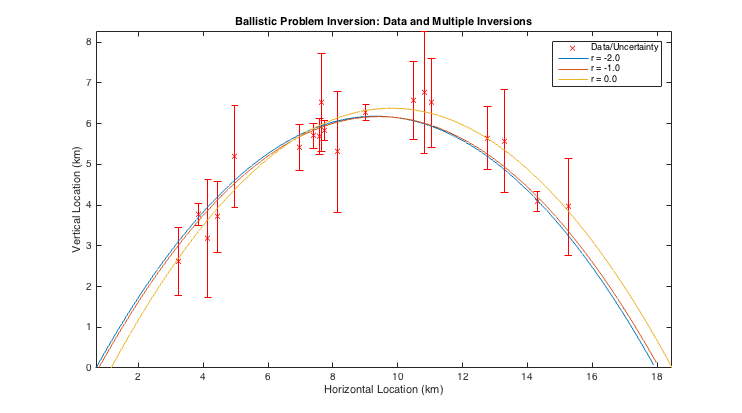
\includegraphics[width=\textwidth]{Ballistic.png}
\end{figure}
\begin{center}
\begin{tabular}{|c|rrrr|}
\hline
Color & $x_{0}$ (km) & $\|\vec{v_{o}}\|$ $\frac{km}{sec}$ & $\theta$ (deg) & $n$ \\
\hline
\rule{0pt}{3ex} Blue & $0.69428$ & $0.42461$ & $55.087$ & $2.0$ \\
Orange & $0.77719$ & $0.42461$ & $54.9834$ & $1.0$ \\
Yellow (Unweighted) & $1.1592$ & $0.42744$ & $55.8294$ & $0.0$ \\
\hline
\end{tabular}
\end{center}
This plot shows that although weighting the data differently affects the parabola, all three scenarios generally achieve the same result. Minimizing the residuals in the ballistic problem is an effective way to solve for the the model parameters $a$, $b$, and $c$ or $x_{o}$, $\|\vec{v_{o}}\|$, and $\theta$ which define the trajectory of the ballistic object.

\pagebreak
\section*{Appendix I: The Code}
\begin{verbatim}
function HW1(filename)
    data = importdata(filename);
    figure;
    errorbar(data(:, 1),data(:, 2),data(:, 3),'rx');
    hold on;
    Weighted_Ballistic_Inversion(data(:, 1), data(:, 2), data(:, 3), 2.0);
    Weighted_Ballistic_Inversion(data(:, 1), data(:, 2), data(:, 3), 1.0);
    Weighted_Ballistic_Inversion(data(:, 1), data(:, 2), data(:, 3), 0.0);
    legend('Data/Uncertainty', 'r = 2.0', 'r = 1.0', 'r = 0.0');
    title('Ballistic Problem Inversion: Data and Multiple Inversions');
    xlabel('Horizontal Location (km)');
    ylabel('Vertical Location (km)');
end

function [m] = Weighted_Ballistic_Inversion(h, z, w, p)
    W = diag((w.^(-p)));
    G = ones(length(h), 3);
    G(:, 2) = G(:, 2) .* h;
    G(:, 3) = G(:, 3) .* (h .^ 2);
    m = pinv((G.')*(W.')*(W)*(G))*(G.')*(W.')*(W)*(z);
    r = roots([m(3) m(2) m(1)]);
    x = r(2):0.1:r(1);
    y = m(1).*ones(1, length(x)) + m(2).*x + m(3).*(x.^2);
    x0 = r(2);
    theta = atan(m(2)+(2.*m(3).*x0));
    vel = ((-9.81*(10^(-3)))./((2.0).*m(3).*(cos(theta).^2))).^0.5;
    display(['X initial (km): ', num2str(x0)]);
    display(['Theta (deg): ', num2str(theta.*180./(3.1415926))]);
    display(['Velocity (km/s): ', num2str(vel)]);
    plot(x, y);
    axis tight;
    hold on;
end
\end{verbatim}

\end{document}